\begin{figure*}
    \centering
    \makebox[\textwidth][c]{%
    \begin{minipage}{6.5in}
        \centering
        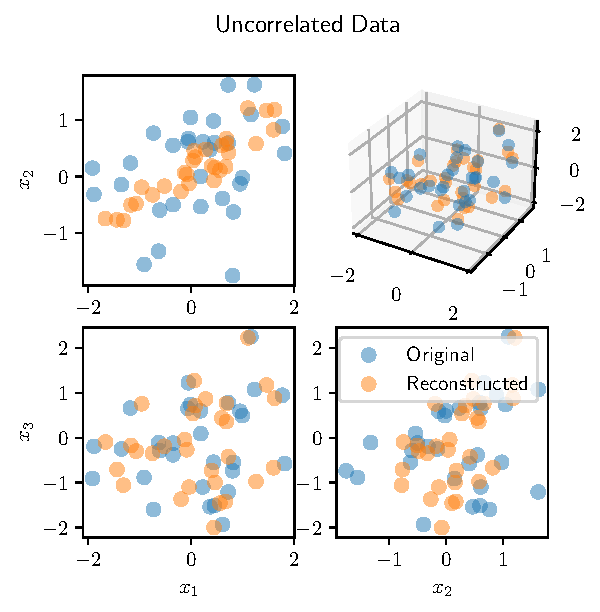
\includegraphics[width=.49\textwidth]{figs/fig-pca-code-uncorr.pdf}
        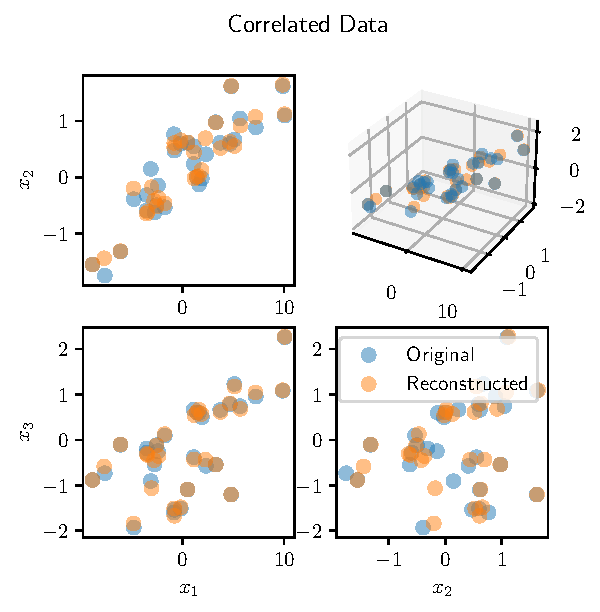
\includegraphics[width=.49\textwidth]{figs/fig-pca-code-corr.pdf}
    \end{minipage}}
    \caption{PCA projection of three-dimensional data onto two-dimensional subspace.}
    \label{fig:pca-code}
\end{figure*}
In the following experiment, we consider two sets of three-dimensional data.
Each set of vectors \(x_1, x_2, x_3 \in \RR^n\) are sampled from a standard normal distribution with sample size \(n = 30\).
Suppose in the first set there is no apparent relationship among variables while, in second set, we have \(x_1 = 4x_2 + 2x_3\).
For simplicity, we say the first set is \textit{uncorrelated} while the second set is \textit{correlated}.
See \Cref{fig:pca-code}.
In the uncorrelated data, the reconstruction error is \(~ 3.92\), which does not seem to indicate the presence of a pattern.
The reconstruction error for the correlated data is \(~ 0.973\).
This error can be explained by the variation of \(x_2\) with \(x_3\).
Meanwhile, the correlated pair plots indicate a pattern among \(x_2\) vs \(x_1\) and \(x_3\) vs \(x_1\).